
\chapter{Networking Foundations}

\section{Introduction to Networking}

Networking is the practice to connect multiple devices together to share resources and informations. It is the foundation of the internet and also the backbone of cloud computing. When a device needs to communicate with another one it splits data into packets with an header and sends them over the network. The packets are then reassembled at the destination device. This process is called packet switching.

\subsection{The 5-Layer Network Model}

The network model is characterized by layered architecture which splits networking into different levels of abstraction, each one with a specific purpose. This architecture is called the network model and it is used to standardize network communications.

The \textbf{OSI network model} is the most common model used in networking and it is composed by 7 layers. The \textbf{5-layer model} is a simplified version and it is composed by the following layers:

{
    \usetikzlibrary{positioning}

    \tikzset{
        box/.style={draw, rectangle, minimum width=4cm, minimum height=1cm, align=center},
        textlabel/.style={align=center, font=\Large},
        smalltext/.style={},
    }

    \hfill
    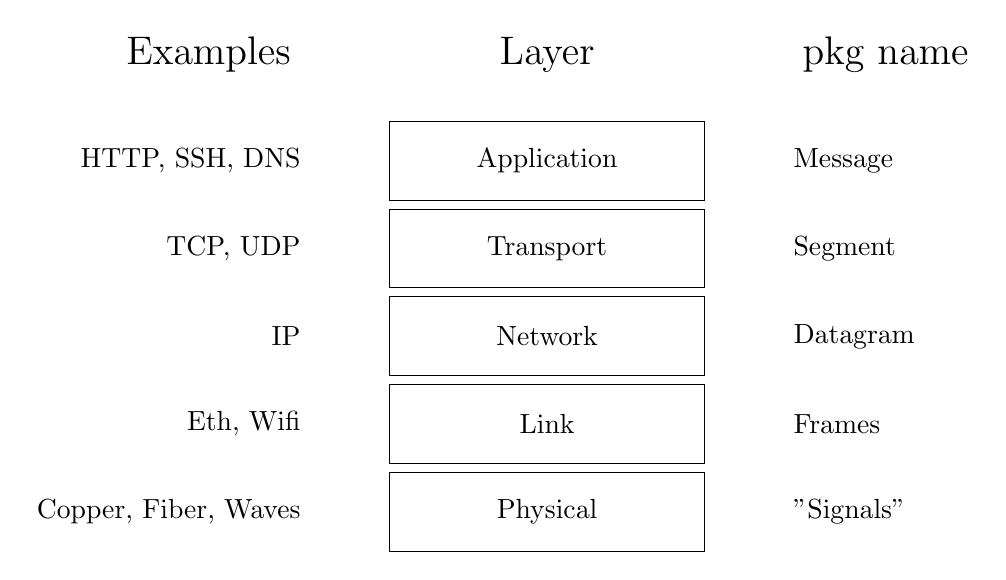
\begin{tikzpicture}[node distance=0.1cm and 2cm]

        % Colonne con etichette
        \node[textlabel, anchor=south] (examples) at (-4.3, 6) {Examples};
        \node[textlabel, anchor=south] (layer) at (0, 6) {Layer};
        \node[textlabel, anchor=south] (pkgname) at (4.3, 6) {pkg name};

        % Layer boxes
        \node[box] (app) at (0, 5) {Application};
        \node[box, below=of app] (transport) {Transport};
        \node[box, below=of transport] (network) {Network};
        \node[box, below=of network] (link) {Link};
        \node[box, below=of link] (physical) {Physical};
        
        % Left column (Examples)
        \node[smalltext, left=1cm of app] (ex1) {HTTP, SSH, DNS};
        \node[smalltext, left=1cm of transport] (ex2) {TCP, UDP};
        \node[smalltext, left=1cm of network] (ex3) {IP};
        \node[smalltext, left=1cm of link] (ex4) {Eth, Wifi};
        \node[smalltext, left=1cm of physical] (ex5) {Copper, Fiber, Waves};
        
        % Right column (pkg name)
        \node[smalltext, right=1cm of app] (pkg1) {Message};
        \node[smalltext, right=1cm of transport] (pkg2) {Segment};
        \node[smalltext, right=1cm of network] (pkg3) {Datagram};
        \node[smalltext, right=1cm of link] (pkg4) {Frames};
        \node[smalltext, right=1cm of physical] (pkg5) {"Signals"};
        
        % Aggiunta di linee di collegamento invisibili per allineare il testo
        \draw[opacity=0] (examples) -- (app);
        \draw[opacity=0] (pkgname) -- (app);
        
    \end{tikzpicture}
    \hfill
}

Each layer in the network model combines software and hardware differently. Application and Transport layers run primarily as software on end devices and servers, enabling flexible protocol updates. The Network layer uses a hybrid approach with software routing and hardware-accelerated forwarding. Physical and Data Link layers are mainly hardware-based, implemented in NICs and transmission media for optimal performance.

While this layered architecture promotes modularity and easier maintenance, it can introduce overhead due to data encapsulation and occasional duplication of functionality across layers. Some modern approaches, like Software-Defined Networking (SDN), attempt to optimize these trade-offs by allowing more flexible layer interactions.

\subsubsection{Physical Layer (L1)} \label{layer1}

The physical layer is the lowest layer of the network model and it is responsible for the physical connection between devices. It defines the hardware and the physical medium used to transmit data. The physical layer is responsible for the transmission of raw data bits over a physical medium.

\subsubsection{Data Link Layer (L2)} \label{layer2}

The data link layer is responsible for reliable point-to-point delivery of data frames between directly connected nodes. It handles addressing using MAC (Media Access Control) addresses, error detection, and flow control. This layer breaks data into frames and ensures reliable transmission over a single network segment. Common protocols at this layer include Ethernet for wired networks and Wi-Fi (802.11) for wireless networks.

The data link layer also manages access to the shared physical medium through protocols like CSMA/CD (Carrier Sense Multiple Access with Collision Detection) for Ethernet or CSMA/CA (Carrier Sense Multiple Access with Collision Avoidance) for wireless networks. For more information on MAC addressing, refer to Section~\ref{mac_addr}.

\subsubsection{Network Layer (L3)}
\label{layer3}

The network layer manages the routing and forwarding of data across the network. It ensures that packets are sent from the source to the destination, potentially through multiple routers. The network layer uses IP addresses to determine the best path for packet delivery. For a more detailed analysis of IP addressing, refer to Section~\ref{ip_addr}.

\subsubsection{Transport Layer (L4)} \label{layer4}

The \textbf{transport layer} is responsible for end-to-end communication between applications. It includes two primary protocols:

\begin{itemize}
    \item \textbf{UDP} (\textit{User Datagram Protocol}): A connectionless, unreliable protocol typically used for applications requiring fast, continuous data transmission, such as audio and video streaming. It does not guarantee delivery or order but is faster than TCP.

    UDP uses only the \textbf{destination IP} and \textbf{destination port}. It is simpler than TCP, as it does not establish a persistent connection. This makes UDP faster but less reliable, with no need for tracking the source address once the data is sent.

    \item \textbf{TCP} (\textit{Transmission Control Protocol}): A connection-oriented, reliable protocol used for most types of data transfer. It ensures data is delivered in order and without errors, making it suitable for tasks like file transfers and web browsing.

    TCP requires more detailed parameters, including both the \textbf{source IP} and \textbf{source port} in addition to the \textbf{destination IP} and \textbf{destination port}. These allow for two-way communication and reliable delivery of data, as TCP establishes and maintains a connection between sender and receiver.
\end{itemize}

\subsubsection{Application Layer (L5)} \label{layer5}

The application layer is the top layer in the network protocol stack, where user-facing applications interact with the network. It provides protocols, such as HTTP, SMTP, and FTP, to facilitate services like web browsing, email, and file transfer. This layer handles high-level communication between software applications and enables them to exchange data over a network.

The \textbf{Domain Name System} (DNS) translates human-readable hostnames (e.g. www.example.com) into IP addresses that computers use to identify each other on the network. It acts as the internet's phonebook, ensuring users can access websites and services without needing to remember numerical addresses. A \textbf{socket} is an endpoint for communication between two machines over a network. It combines an IP address and a port number to establish a connection, allowing applications to send and receive data.

\begin{neonlisting}[language=Python]{Socket creation: Client}
# Socket creation
clientSocket = Socket(AF_INET, SOCK_STREAM)
# socket connection opening
clientSocket.connect((server_name, server_port))
\end{neonlisting}

\begin{neonlisting}[language=Python]{Socket creation: Server}
# Socket creation
clientSocket = Socket(AF_INET, SOCK_STREAM)
# socket start listening
clientSocket.bind(('', server_port))
clientSocket.listen(1)
\end{neonlisting}

\subsection{Data Encapsulation} \label{encapsulation}

\textbf{Data encapsulation} is the process of wrapping data with necessary protocol information before network transmission. Each layer of the network model adds its own \textbf{header} (and sometimes \textbf{trailer}) to the data from the layer above, creating a packet that can be properly routed and delivered (\cref{fig:encapsulation}). This encapsulation ensures that data is transmitted accurately and efficiently across the network, with each layer handling specific aspects of the communication process. The actual data in a packet is called \textbf{payload}.

\begin{figure}[H]
    \centering
    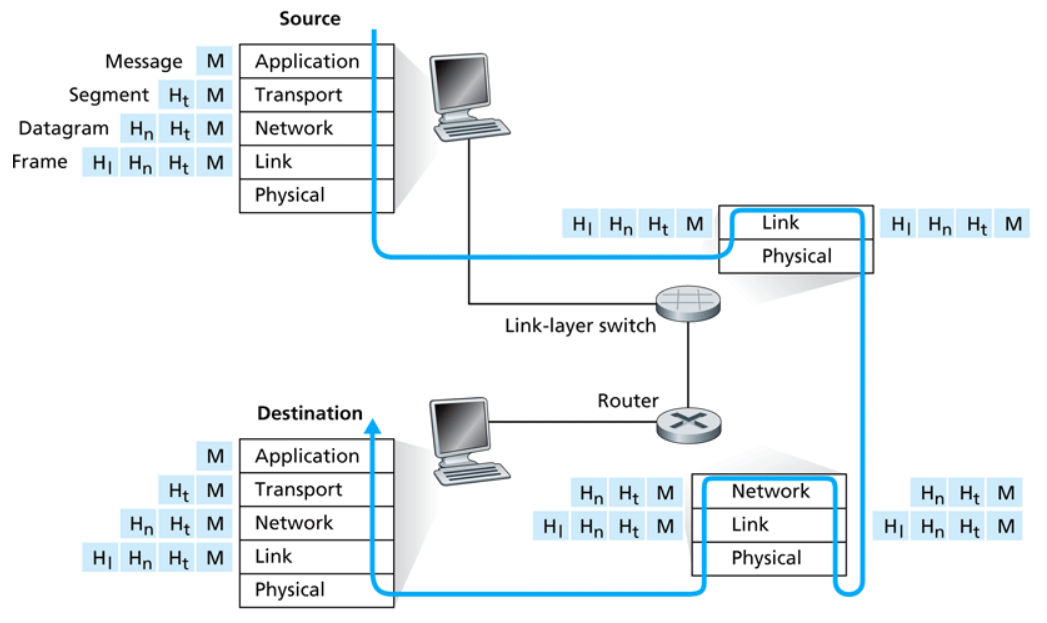
\includegraphics[scale=0.4]{assets/encapsulation.png}
    %\captionsetup{justification=centering}
    \caption{Encapsulation path} \label{fig:encapsulation}
\end{figure}

Each layer's headers (and trailers) contain data specific to the protocol operating at that layer. For example, the network layer header includes source and destination IP addresses, while the transport layer header includes source and destination port numbers. They can also include error detection bits that allow the receiver to determine if any bits in the message have changed during transit. This layered approach allows each protocol to focus on its specific function, ensuring modularity and ease of troubleshooting.

\section{Network Addressing} \label{addressing}

Efficient network communication relies on a robust addressing mechanism to ensure data packets are delivered to their intended destinations. The process begins with setting the correct destination address, followed by forwarding the packet through routers using MAC addresses at Layer 2. Routers, equipped with forwarding tables, determine the optimal path for each packet, mapping destination addresses to specific link interfaces.

In layer 3, the Internet model adopts a "best-effort" delivery approach. This design does not guarantee timing, order, or delivery of packets, but it prioritizes flexibility and scalability across vast and interconnected networks. Additional controls, such as ensuring reliability and sequencing, are delegated to higher layers within the protocol stack, allowing the network layer to focus on efficient routing and addressing.

\subsection{MAC and IP Addressing}

\subsubsection{MAC addressing} \label{mac_addr}

A MAC address is a unique identifier for each network interface on a device. These addresses operate at the \hyperref[layer2]{link layer} (L2), enabling local communication between devices. The address FF:FF:FF:FF:FF:FF is used for broadcasting to all devices on a network.

The Address Resolution Protocol (ARP) is used to map an IP address to a MAC address on a local network. When a device needs to communicate with another device within the same network segment, it sends an ARP request to determine the corresponding MAC address.

\subsubsection{IP Addressing} \label{ip_addr}

The \textbf{Internet Protocol (IP)} is a fundamental protocol within the Internet protocol suite, responsible for addressing and routing packets of data so they can traverse interconnected networks and reach their intended destinations. Operating at the \hyperref[layer3]{network layer} (L3), IP ensures that data sent from a source device is directed toward the correct recipient through various networking devices such as routers and switches.

The IPv4 datagram (\cref{fig:datagram}) includes important fields like the version, header length, flags for fragmentation, source and destination IP addresses, and other optional fields. It allows for routing and addressing across the network. Key fields include:

\begin{itemize}
    \item Version (IPv4 or IPv6).
    \item Flags for managing fragmentation.
    \item Source and destination IPs that identify the sender and receiver.
    \item Upper-layer protocol (such as TCP or UDP) used to transport the data.
\end{itemize}

\begin{figure}[H]
    \centering
    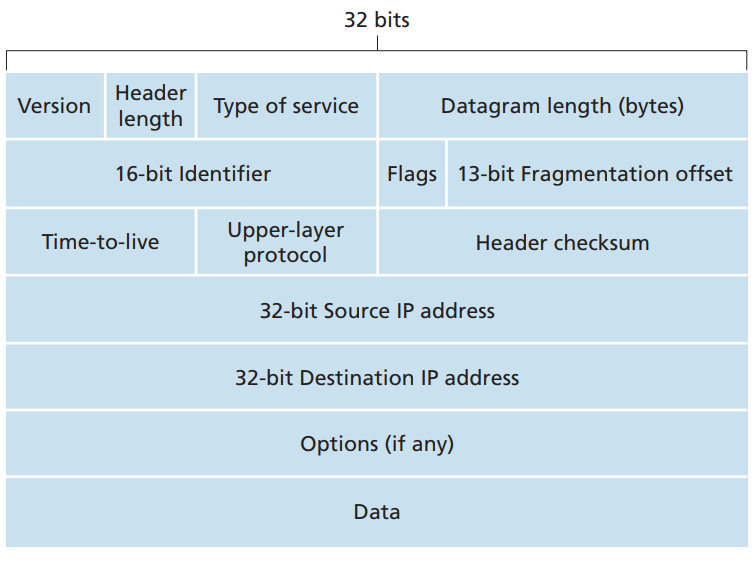
\includegraphics[scale = 0.4]{assets/datagram.png}
    \caption{IPv4 datagram structure} \label{fig:datagram}
\end{figure}

An IPv4 address is a 32-bit number divided into four octets, each representing a decimal number (e.g., 172.16.254.1). The address is used to uniquely identify a device on a network, typically paired with a subnet mask (e.g., /24) to define the network range.

\observationblock[IPv6]{
    While these notes focus on IPv4 addressing and datagrams, it is important to acknowledge the growing significance of \textbf{IPv6} in modern networking. IPv6, with its 128-bit address space, was designed to address the limitations of IPv4, particularly the exhaustion of available addresses. Although not covered here, further exploration of IPv6 is recommended for a comprehensive understanding of contemporary network protocols.
}

\subsection{Hostnames and DNS}
\label{hostnames_dns}

\textbf{Hostnames} are human-readable labels assigned to devices on a network, facilitating easier identification and access compared to numerical IP addresses. For example, \texttt{www.example.com} is more memorable than its corresponding IP address.

The \textbf{Domain Name System (DNS)} is a hierarchical service that translates hostnames into IP addresses, enabling users to access resources using familiar names. When a user enters a hostname into a browser, a DNS query resolves it to the appropriate IP address, allowing the connection to be established seamlessly. DNS can be vulnerable to attacks like DNS spoofing and cache poisoning. Security measures like DNSSEC help ensure DNS response integrity and authenticity.

\subsection{Network Ports}
\label{network_ports}

\textbf{Network ports} are logical endpoints used by the Transport Layer protocols (TCP and UDP) to differentiate between multiple services running on a single device. Each port is identified by a unique number ranging from 0 to 65535.

Well-known ports (0-1023) are reserved for common services such as HTTP (\texttt{80}), HTTPS (\texttt{443}), and SSH (\texttt{22}). Registered ports (1024-49151) are assigned to user applications and services, while dynamic or private ports (49152-65535) are typically used for temporary communications initiated by client applications.

Proper management of network ports is crucial for both functionality and security. Open ports can be potential entry points for unauthorized access, making it important to monitor and control port usage through firewalls and security policies.

\warningblock[Port Security]{
    Unsecured open ports can be exploited by malicious actors to gain unauthorized access or disrupt services. Regularly auditing open ports and implementing strict firewall rules are essential practices to protect network integrity.
}

\subsection{Core Network Services}
\label{core_network_services}

\subsubsection{CIDR}
\label{cidr}

\textbf{Classless Inter-Domain Routing (CIDR)} notation enhances IP address allocation by using the format \texttt{a.b.c.d/x}, where \texttt{x} indicates the number of bits in the network prefix. Introduced to improve the scalability of IP addressing, CIDR allows for more flexible and efficient use of IP address spaces compared to the traditional class-based system. By aggregating IP addresses into variable-length blocks, CIDR reduces the size of routing tables and optimizes routing efficiency.

\exampleblock[CIDR Notation Example]{
    Consider the network 192.168.1.0/24:
    \begin{itemize}
        \item Network address: 192.168.1.0
        \item Subnet mask: 255.255.255.0
        \item First usable IP: 192.168.1.1
        \item Last usable IP: 192.168.1.254
        \item Broadcast address: 192.168.1.255
        \item Total IPs: 256 (254 usable)
    \end{itemize}
    $\\$
    Another example with 192.168.0.0/16:
    \begin{itemize}
        \item Network range: 192.168.0.0 to 192.168.255.255
        \item Subnet mask: 255.255.0.0
        \item Total IPs: 65,536 (65,534 usable)
    \end{itemize}
}

\subsubsection{NAT}
\label{nat}

\textbf{Network Address Translation (NAT)} enables multiple devices on a local network to share a single public IP address. By translating private IP addresses to a public address using a translation table, NAT conserves the limited pool of public IP addresses and provides a layer of security by obscuring internal network structures from external entities.

\begin{figure}[H]
    \centering
    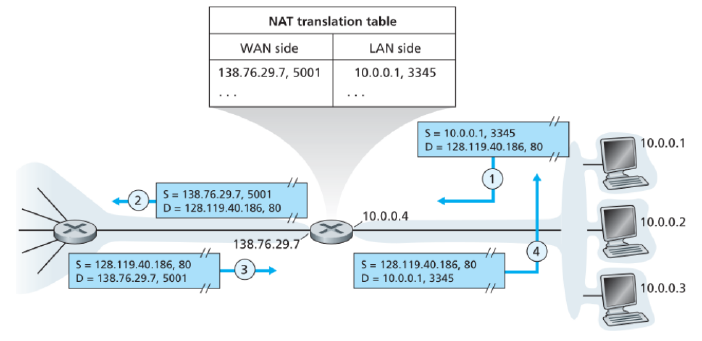
\includegraphics[scale=0.4]{assets/nat.png}
    \caption{Network Address Translation (NAT) Process}
    \label{fig:nat_process}
\end{figure}

\observationblock[NAT and IPv6]{
    While NAT has been instrumental in conserving IPv4 addresses, the adoption of \textbf{IPv6} eliminates the need for NAT by providing a vast address space. IPv6 allows for direct end-to-end connectivity, simplifying network configurations and improving performance.
}

\subsubsection{DHCP}
\label{dhcp}

\textbf{Dynamic Host Configuration Protocol (DHCP)} automates the assignment of IP addresses and other network configurations to devices on a network. As shown in \cref{fig:dhcp_process} when a device connects, it sends a DHCP request, and a DHCP server responds with an available IP address, subnet mask, default gateway, and DNS server information.

\begin{figure}[H]
    \centering
    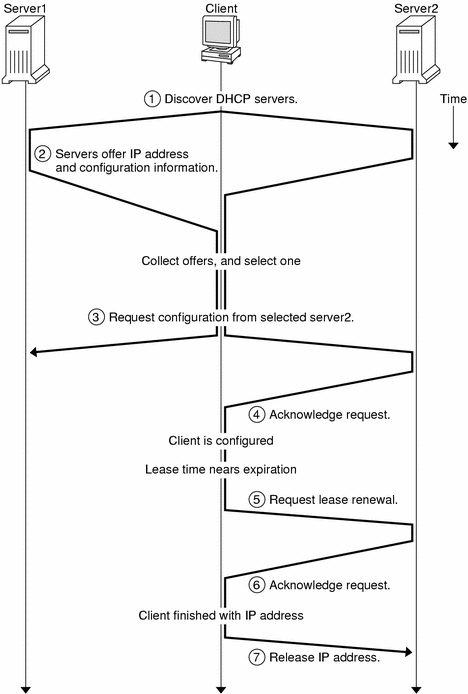
\includegraphics[scale=0.4]{assets/dhcp.png}
    \caption{DHCP Process Flow}
    \label{fig:dhcp_process}
\end{figure}

DHCP simplifies network management by dynamically allocating IP addresses, reducing the likelihood of address conflicts, and allowing for efficient utilization of IP address pools.
